% !TeX root = SA_Rockstroh_Main.tex
\chapter{Katalog von Modellen der Regelungstechnik}
\label{Ch:Ergebnisse}
% Ziel/Inhalt: Nur die Ergebnisse und keine großartigen Begründungen. Die sollen prinzipiell alle im vorherigen Kapitel stehen.
In diesem Kapitel werden die Ergebnisse der Studienarbeit vorgestellt. Angefangen wird mit der Struktur des Kataloges. Danach werden das Klassifikationssystem(s. \ref{Ch:Ergebnisse:Sec:KS}), die Modelldokumentation(s. \ref{Ch:Ergebnisse:Sec:Dokumentation}) und die Modellimplementation(s. \ref{Ch:Ergebnisse:Sec:Implementation}) als wichtige Elemente des Kataloges beschrieben. Eine Auflistung der aktuell vorhandenen Modelle(s. \ref{Ch:Ergebnisse:Sec:Modelle}) und eine Beschreibung des Ablaufes der Katalogerweiterung(s. \ref{Ch:Ergebnisse:Sec:Erweiterung}) schließen das Kapitel ab.
% Alternative Einführung: Like KS - Beschreibung was der Katalog ist.
% Einschub zur Terminologie: Etwas wird gemacht - ist schon umgesetzt. Etwas soll gemacht werden - noch nicht umgesetzt/praktiziert.
% ===========================================
% ------------- Katalogstruktur -------------
% ===========================================
\section{Katalogstruktur}
\label{Ch:Ergebnisse:Sec:Struktur}
Der Katalog besteht aus folgenden Elementen: Dem \textit{Klassifikationssystem}, dem Python Package \textit{GeneralModel} und Modelleinträgen, die aus einer \textit{Metadaten-Datei}, der \textit{Modelldokumentation}, einer \textit{Parameter-Datei} und, optional, aus der implementierten \textit{Modellklasse} bestehen. Für jede Datei der Modelleinträge gibt es eine Vorlage. Die Beziehungen zwischen den Elementen sind in \autoref{fig:Katalogstruktur}dargestellt.

%\ref{fig:Katalogstruktur} 
%BILD: Katalogstruktur
%=====================
\begin{figure}[H]
	\centering
	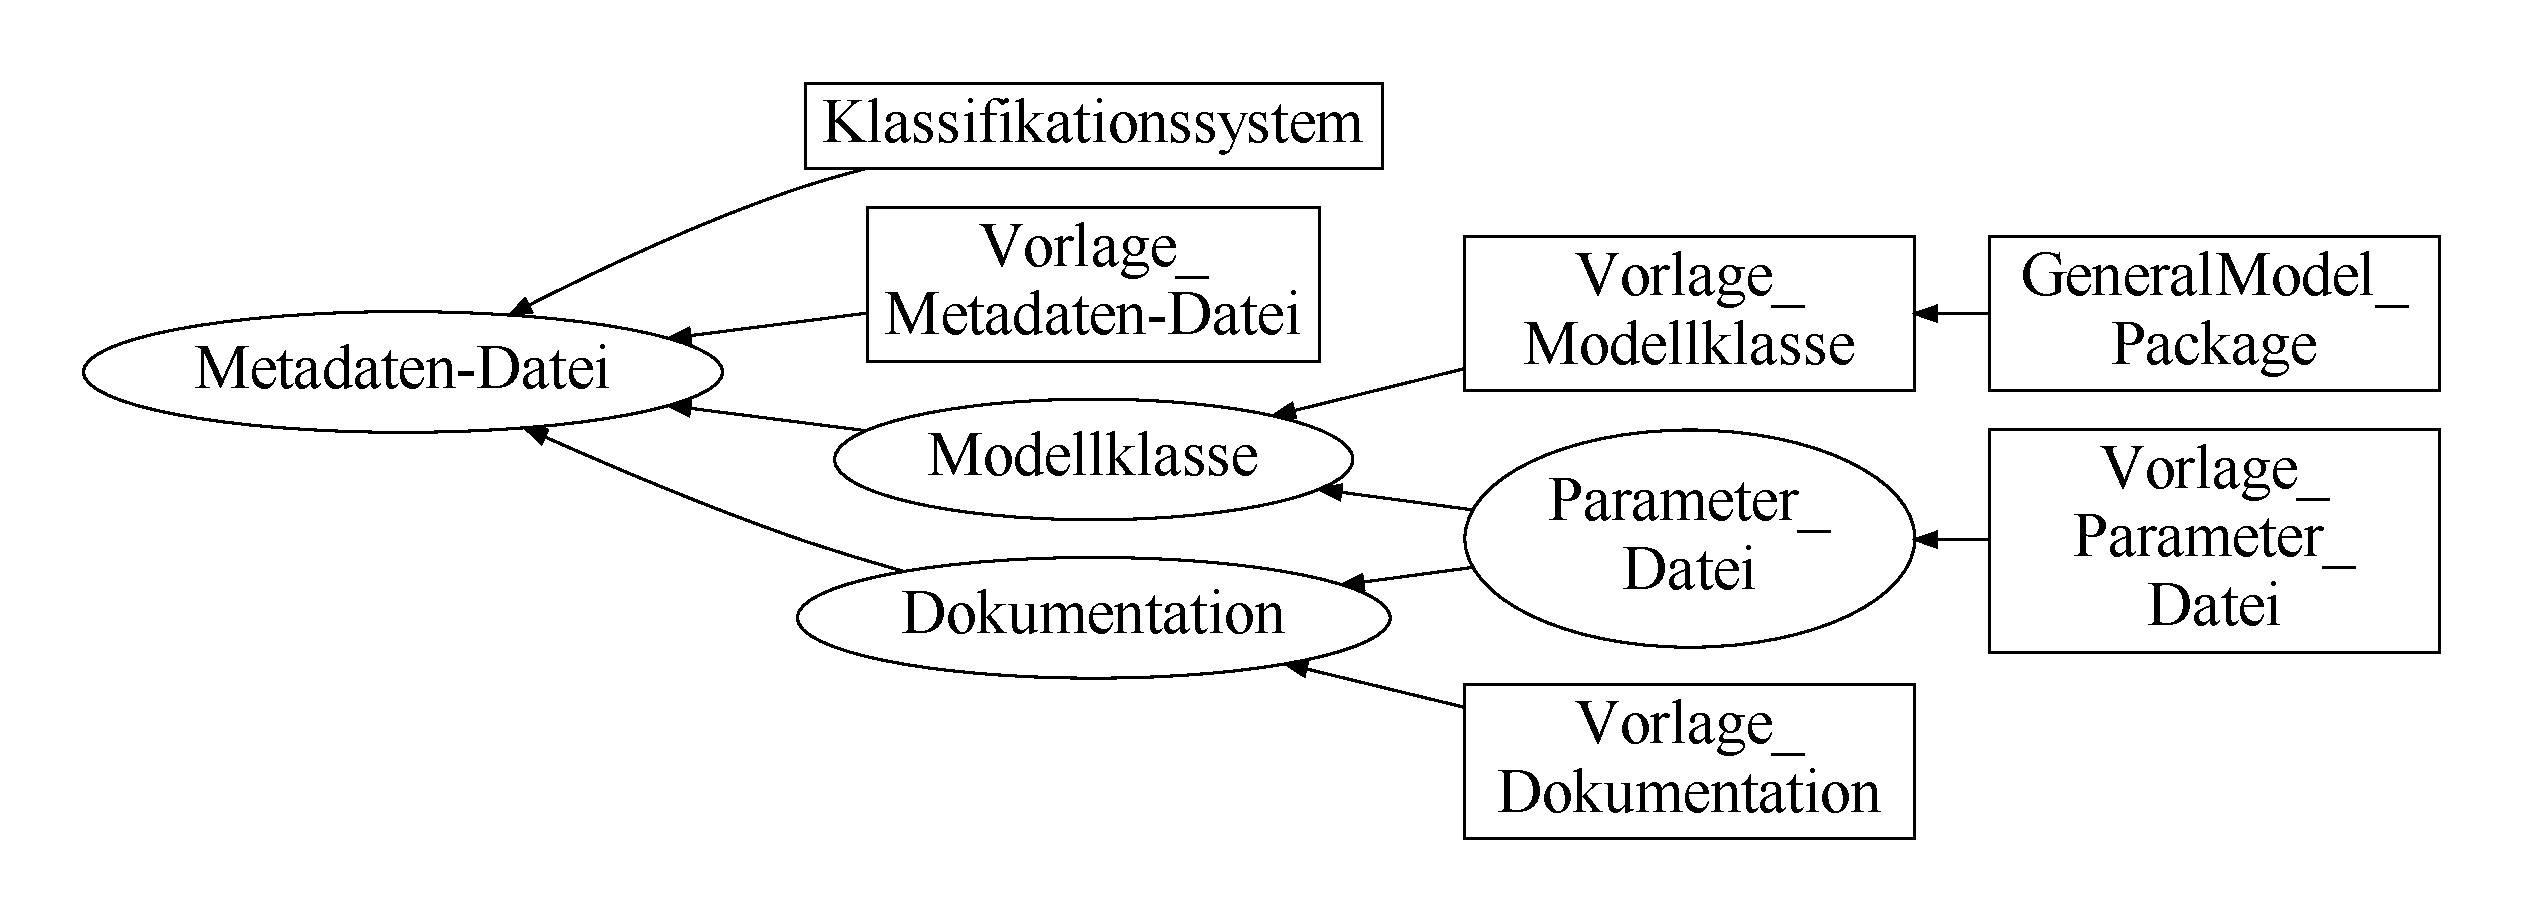
\includegraphics[width=1\linewidth]{Katalogstruktur}
	\caption[Katalogstruktur]{Elemente in Ellipsen existieren individuell für jedes Modell. Elemente in Rechtecken existieren genau ein Mal im Katalog.}
	\label{fig:Katalogstruktur}
\end{figure}

Das \textit{Klassifikationssystem} ist eine Übersicht der Modelleigenschaften und deren Beziehungen untereinander. Die Einträge in dem Feld für die Modelleigenschaften in der Metadaten-Datei(\textit{tag\_list}) sind nur Namen von Kategorieknoten aus dem KS. Es sorgt für eine einheitliche Namensgebung der Modelleigenschaften(s. Anforderung \ref{A.Modelleigenschaften}). 

Das Python Package \textit{GeneralModel} stellt die Python Klasse \textit{GeneralModel} zur Verfügung, von der alle Modellklassen der implementierten Modelle erben. Sie stellt ein Variablen- und Methodenset bereit, das alle Modellklassen gemeinsam haben.

Die \textit{Metadaten-Datei} ist eine Datei im YAML-Format, das Informationsfelder für Informationen zu dem zugehörigen Modell enthält. Es gibt Felder für Informationen\dots 
\begin{itemize}[label=$\bullet$]
	\item über das Modell (Modellname, Kurzbeschreibung, Modelleigenschaften, Dateinamen der Modellbilder)
	\item für eine Umsetzung des Kataloges als Datenbank(Key, Predecessor-Key, Implementation-Key)
	\item anderer Art (Modellersteller, Erstellungsdatum, Liste der Bearbeiter, Externe Referenzen)
\end{itemize}
Das Konzept und die Umsetzung der Metadaten-Datei stammt aus dem \textit{ACKRep}\footnote{ACKRep GitHub Repository: https://github.com/ackrep-org/ackrep\_data}.
% Noch schreiben welche Informationen im aktuellen Stand gegeben werden?

Die \textit{Modelldokumentation} ist die textuelle Notation des Modells. Sie wird in \LaTeX  geschrieben. Nach jeder Bearbeitung wird die PDF-Datei aus der \LaTeX-Datei erzeugt. 

Die \textit{Parameter-Datei} ist eine Python-Datei. Diese enthält beispielhafte Parameterwerte für das Modell. Das Ausführen der Datei erzeugt eine Tabelle mit den beispielhaften Parameterwerten im \LaTeX-Format, schreibt diese in eine Datei Namens \textit{Parameter.tex} und speichert die Datei im Ordner der Modelldokumentation. Außerdem stellt Sie eine Methode für die implementierte Modellklasse bereit, welche die Parameter des Modells als Rückgabewert hat.

Die implementierte \textit{Modellklasse} ist eine Python-Datei, welche das Modell als Python-Klasse enthält. 

Die \textit{Vorlagen} für die Metadaten-Datei, die Parameter-Datei, die Modelldokumentation und -implementation sind Dateien, welche den Arbeitsaufwand für das Anlegen neuer Modelle verringern sollen(siehe Entscheidung \ref{E.Vorlagen}). Die repetitiven Elemente für die entsprechenden Dateien sind in den Vorlagen schon vorhanden, so dass nur die Modellspezifischen Elemente neu geschrieben werden müssen. Die Verwendung der Vorlagen stellt eine einheitliche Struktur der Dateien sicher.

% =================================================
% ------------- Klassifikationssystem -------------
% =================================================
\section{Klassifikationssystem}
\label{Ch:Ergebnisse:Sec:KS}
Das \textit{Klassifikationssystem (KS)} stellt eine Wissensrepräsentation dar. Es lehnt stark an die in \cite{KNHE20a} eingeführte \textit{OCSE} an, von der es sich insofern unterscheidet, das im KS nur die Teilbereiche des Wissens der Mathematik, Regelungs- und Steuerungstheorie enthalten sind, die sich auf regelungstechnische Systeme und Modelle beziehen. Die im KS verwendeten Bezeichnungen sollen in den Metadaten-Dateien der Modelle bevorzugt verwendet werden. \\
Es ist anzumerken, dass das KS keine vollständige Wissensrepräsentation darstellt. Das liegt daran, dass das darzustellende Wissen sehr umfangreich ist und eine vollständige Darstellung dessen im Rahmen dieser Studienarbeit nicht schaffbar war. Weiter könnte man auch die Frage stellen, ob überhaupt eine vollständige Darstellung des beabsichtigten Wissensbereiches existiert, da das Wissen dynamisch mit neuen Entdeckungen wächst. Diese Diskussion soll hier aber nicht weitergeführt werden. 

%TODO: Knotenanzahl einfügen
Das KS besteht aktuell aus <Knotenanzahl> Knoten. <Bildreferenz> zeigt ein Ausschnitt des KS.
% =============================================================
% ------------- Aufbau des Klassifikationssystems -------------
% =============================================================
\subsection{Aufbau des Klassifikationssystems}
\label{Ch:Ergebniss:Sec:KS:SubSec:Aufbau}
Das KS ist ein Semantisches Netz(s. \ref{E.KS_SemantischesNetz}), welches durch einen gerichteten, kreisfreien Graphen repräsentiert wird. Es gibt folgende Knotentypen: Kategorie-, Objekt-, Werte, und Wertetypknoten. 
Die Kanten zeigen Beziehungen zwischen den Knoten des KS auf, die durch die Kantenbeschriftungen spezifiziert werden. Es gibt folgende Kantennamen: \glqq is a\grqq, \glqq Value\grqq, \glqq Type\grqq und \glqq Object\grqq. Der Kantenname kennzeichnet zudem den Knotentyp des Startknotens der Kante. Jeder Endknoten einer Kante ist ein Kategorieknoten. Die Beziehung zwischen Knotentypen und Kantennamen wird in der Tabelle \ref{table:KS_KantenUndKnoten} gezeigt.
\begin{table}[H]
	\centering
	\begin{tabular}{l|c|l}
		Startknotentyp & Kantenname & Endknotentyp \\ \hline
		Kategorieknoten & is a & Kategorieknoten \\
		Werteknoten & Value & Kategorieknoten \\
		Wertetypknoten & Type & Kategorieknoten \\
		Objektknoten & Object & Kategorieknoten
	\end{tabular}
	\caption{Beziehung zwischen Kantennamen und Knotentypen}
	\label{table:KS_KantenUndKnoten}
\end{table}

Die Kategorieknoten, außer der Ursprungsknoten und die Knoten der Hauptkategorien, können als Modellattribute interpretiert werden. In der Metadaten-Datei dürfen nur diese Knoten des KS eingetragen werden. \\
Die Kategorieknoten im KS werden durch ihren eindeutigen Namen identifiziert(s. \ref{E.KS_Namensgebung}).\\
Jeder Knoten $k$, außer der Ursprungsknoten, ist entlang eines gerichteten Pfades $P(k)$ mit dem Ursprungsknoten verbunden. Wird einem Modell ein Knoten $k_i$ des KS als Modellattribut zugewiesen, dann hat das Modell auch alle Knoten, außer Ursprungs -und Hauptknoten, entlang des gerichteten $P(k_i)$ als Modellattribut. % Beispiel?

Der Ursprungsknoten \textit{Property\_Of\_Classification\_System} hat die drei Unterkategorien \textit{Property\_Of\_Mathematical\_Representation}, \textit{Model\_Behaviour} und \textit{Usage}. Die Unterkategorien des Ursprungsknoten werden im KS als Hauptkategorien bezeichnet, die jeweils verschiedene Teilmengen von Modellattributen enthalten. Die Hauptkategorien werden wie folgt Beschrieben.

\textbf{Eigenschaften der mathematischen Repräsentation}: \\
Umfasst Eigenschaften der mathematische Repräsentation des Modells.   % ... die aus der math. Rep. direkt hervor gehen. --> Äquivalenzbegriff von Willems

\textbf{Modelleigenschaften}: \\ % Eigenschaften unabhängig von Darstellungsform eines äquivalenten Systems
Umfasst Eigenschaften die aus der mathematischen Repräsentation mit Methoden der Regelungstechnik abgeleitet werden.

\textbf{Verwendung}: \\
Umfasst Aufgabentypen und Anwendungsbereiche in denen die Modelle häufig genutzt werden.

In \ref{Ch:Vorbetrachtung:Sec:SystemeModelle} wurde erwähnt, dass ein Modell mehrere mathematische Repräsentationen haben kann. Dieser Aspekt führt auf den Begriff der \textit{Äquivalenz} zweier mathematischer Modelle. Zwei mathematische Modelle heißen \textit{Äquivalent}, wenn beide das gleiche Set an Trajektorien für ihre externen Variablen zulassen\footnote{vgl. \cite{SCH89}, S. 34}. Oder einfacher, wenn beide Modelle das gleiche dynamische Verhalten aufweisen. Das Modell eines Systems kann durch eine Menge äquivalenter mathematischer Modelle repräsentiert werden. Der Unterschied zwischen den Hauptkategorien \textit{Eigenschaft der mathematischen Repräsentation} und \textit{Modelleigenschaften} liegt darin, dass die Elemente eine Menge äquivalenter mathematischer Modelle die gleichen \textit{Modelleigenschaften} haben, sich aber in ihrer mathematischen Repräsentation unterscheiden.

% ===========================================================================
% ------------- Technische Umsetzung des Klassifikationssystems -------------
% ===========================================================================
\subsection{Technische Umsetzung des Klassifikationssystems}
\label{Ch:Ergebnisse:Sec:KS:SubSec:TechUmsetzung}
Das KS besteht aus vier Dateien im YAML-Format, welche folgende Namen haben: \textit{KS\_Tree\_main}, \textit{KS\_Tree\_Math\_Representation}, \textit{KS\_Tree\_Model\_Attributes} und \textit{KS\_Tree\_Usage}. Die Datei \textit{KS\_Tree\_main} enthält die \textit{Informationsblöcke(IB)} zu dem Ursprungsknoten und den Knoten der Hauptkategorien. Die restlichen drei Dateien enthalten jeweils die Informationsblöcke zu den Knoten der Unterkategorien der Hauptkategorien. \\ 
Ein IB enthält alle Informationen zu genau einem Knoten des KS. Jeder IB in den YAML-Dateien ist ein Mapping. Ein Mapping setzt einen Schlüssel mit genau einem Wert in Beziehung. Das \textit{dictionary} ist das Python-Äquivalent zu einem Mapping in YAML. In einem IB ist der Name des Knotens der Schlüssel und eine Sequenz ist der Wert. \textit{List} und \textit{tuple} sind die Python-Äquivalente zur Sequenz. Jeder Eintrag der Sequenz steht für ein Attribut des Knotens und ist wiederum ein Mapping, dessen Schlüssel der Attributsname und dessen Wert der Attributswert ist. Die IB\grq s sind durch eine Leerzeile voneinander getrennt. Die Abbildung <Abbildungsreferenz> zeigt einige IB\grq s aus der Datei \textit{KS\_Tree\_Math\_Representation}. % vllt noch Hinweis auf einfache Erweiterbarkeit, die durch neue Sequenzeinträge erreicht wird 

Das Python-Script \textit{KS\_Create\_Graph} liest die YAML-Dateien mit Hilfe des Packages \textit{pyyaml}\footnote{Pyyaml Package: https://pyyaml.org/wiki/PyYAMLDocumentation} ein, erzeugt einen Graph des Python Packages \textit{networkx}\footnote{Networkx Package: https://networkx.org/documentation/stable/index.html} und zeichnet den Subgraphen der nur die Kategorieknoten enthält mit dem Python Package \textit{nxv}\footnote{Nxv Package: https://nxv.readthedocs.io/en/latest/index.html} in eine Bilddatei.
% Networkx-Graphen vom Funktionsumfang potenziell als vollständige maschinelle lesbare Repräsentation des KS und dessen Anwendungen auf die Modelle verwendbar

% ===============================================
% ------------- Modelldokumentation -------------
% ===============================================
\section{Modelldokumentation}
\label{Ch:Ergebnisse:Sec:Dokumentation}

% =================================================
% ------------- Modellimplementation  -------------
% =================================================
\section{Modellimplementation}
\label{Ch:Ergebnisse:Sec:Implementation}

% ==============================================
% ------------- Vorhandene Modelle -------------
% ==============================================
\section{Vorhandene Modelle}
\label{Ch:Ergebnisse:Sec:Modelle}

% ==============================================
% ------------- Katalogerweiterung -------------
% ==============================================
\section{Katalogerweiterung}
\label{Ch:Ergebnisse:Sec:Erweiterung}



